%%  Figures of methodology


\begin{figure}
	\centering
	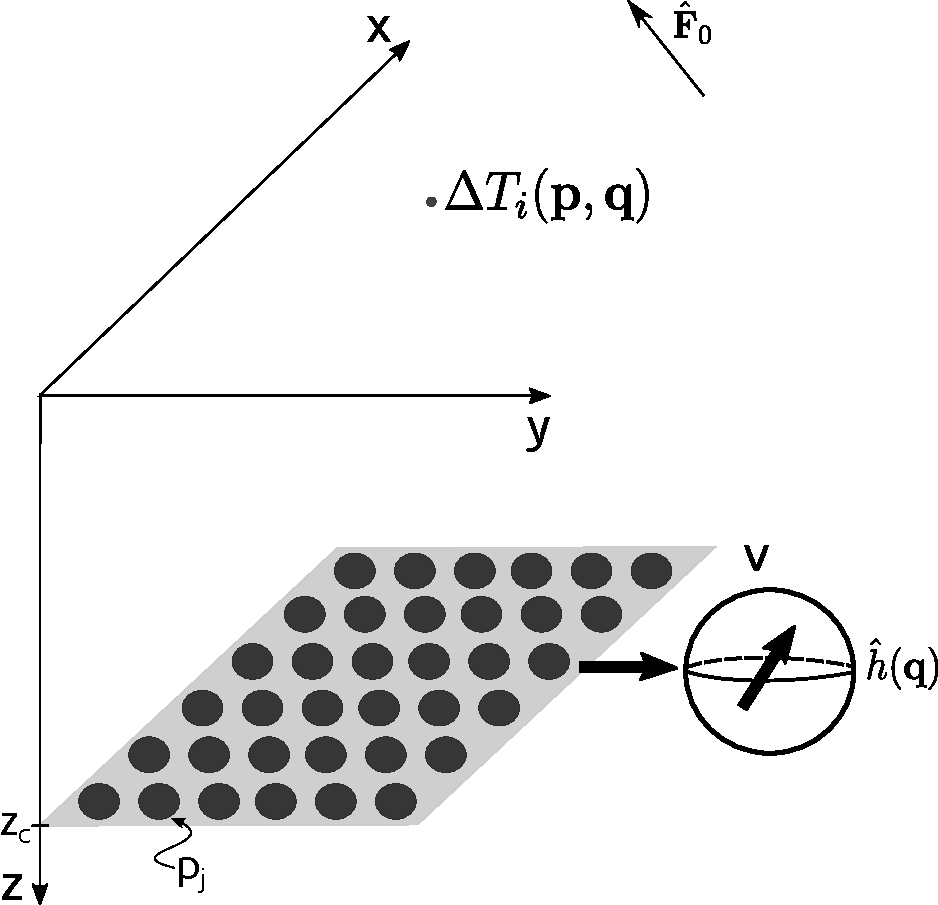
\includegraphics[width=0.7\textwidth]{Fig/eqlayer_figure.pdf}
	\caption{Schematic representation of an equivalent layer. The layer is positioned over the horizontal plane at a depth of $z=z_c$. $\Delta T_i =  f_i (\mathbf{s})$ is the predicted total-field anomaly at the point $(x_i,y_i,z_i)$ produced by the set of $M$ equivalent sources (black dots). Each source is located at the point $(x_j,y_j,z_c)$, $j = 1,\hdots, M$, and represented by a dipole with unity volume $\upsilon$ with magnetization direction $\hat{\mathbf{m}}(\mathbf{q})$ and magnetic moment $p_j$.    }
	\label{fig:eqlayer_figure}
\end{figure}


\begin{figure}
	\centering
	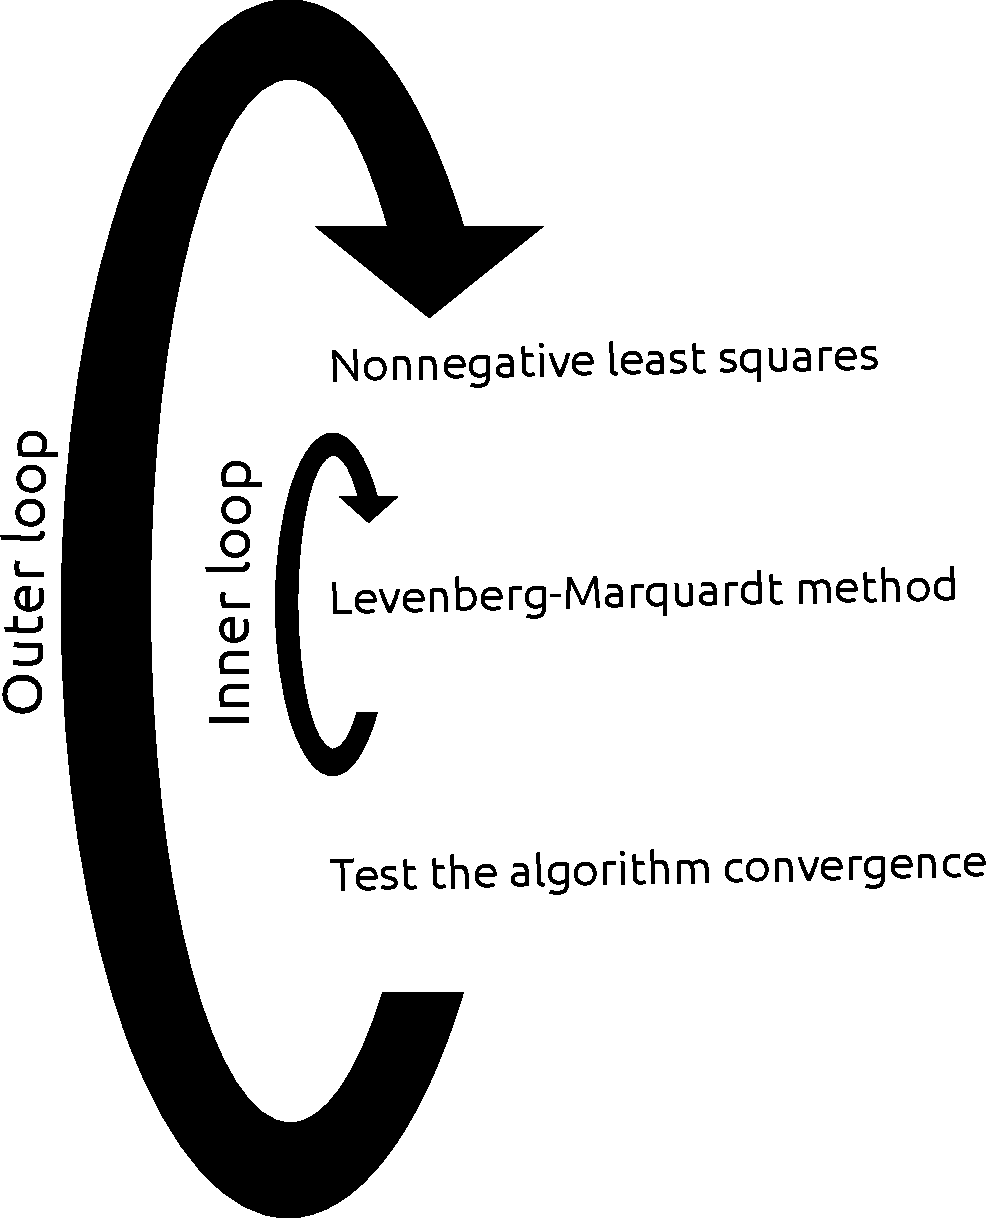
\includegraphics[width=0.6\textwidth]{Fig/algorithm_LM_NNLS.pdf}
	\caption{Iterative scheme overview for NNLS and Levenberg-Marquardt method for estimating magnetization direction. The outer loop is the nonnegative solution for magnetic-moment distribution and the inner loop calculates the magnetization direction correction using Levenberg-Marquardt method.}
	\label{fig:scheme_LM_NNLS}
\end{figure}

%% Figures synthetic tests

\begin{figure}
	\centering
	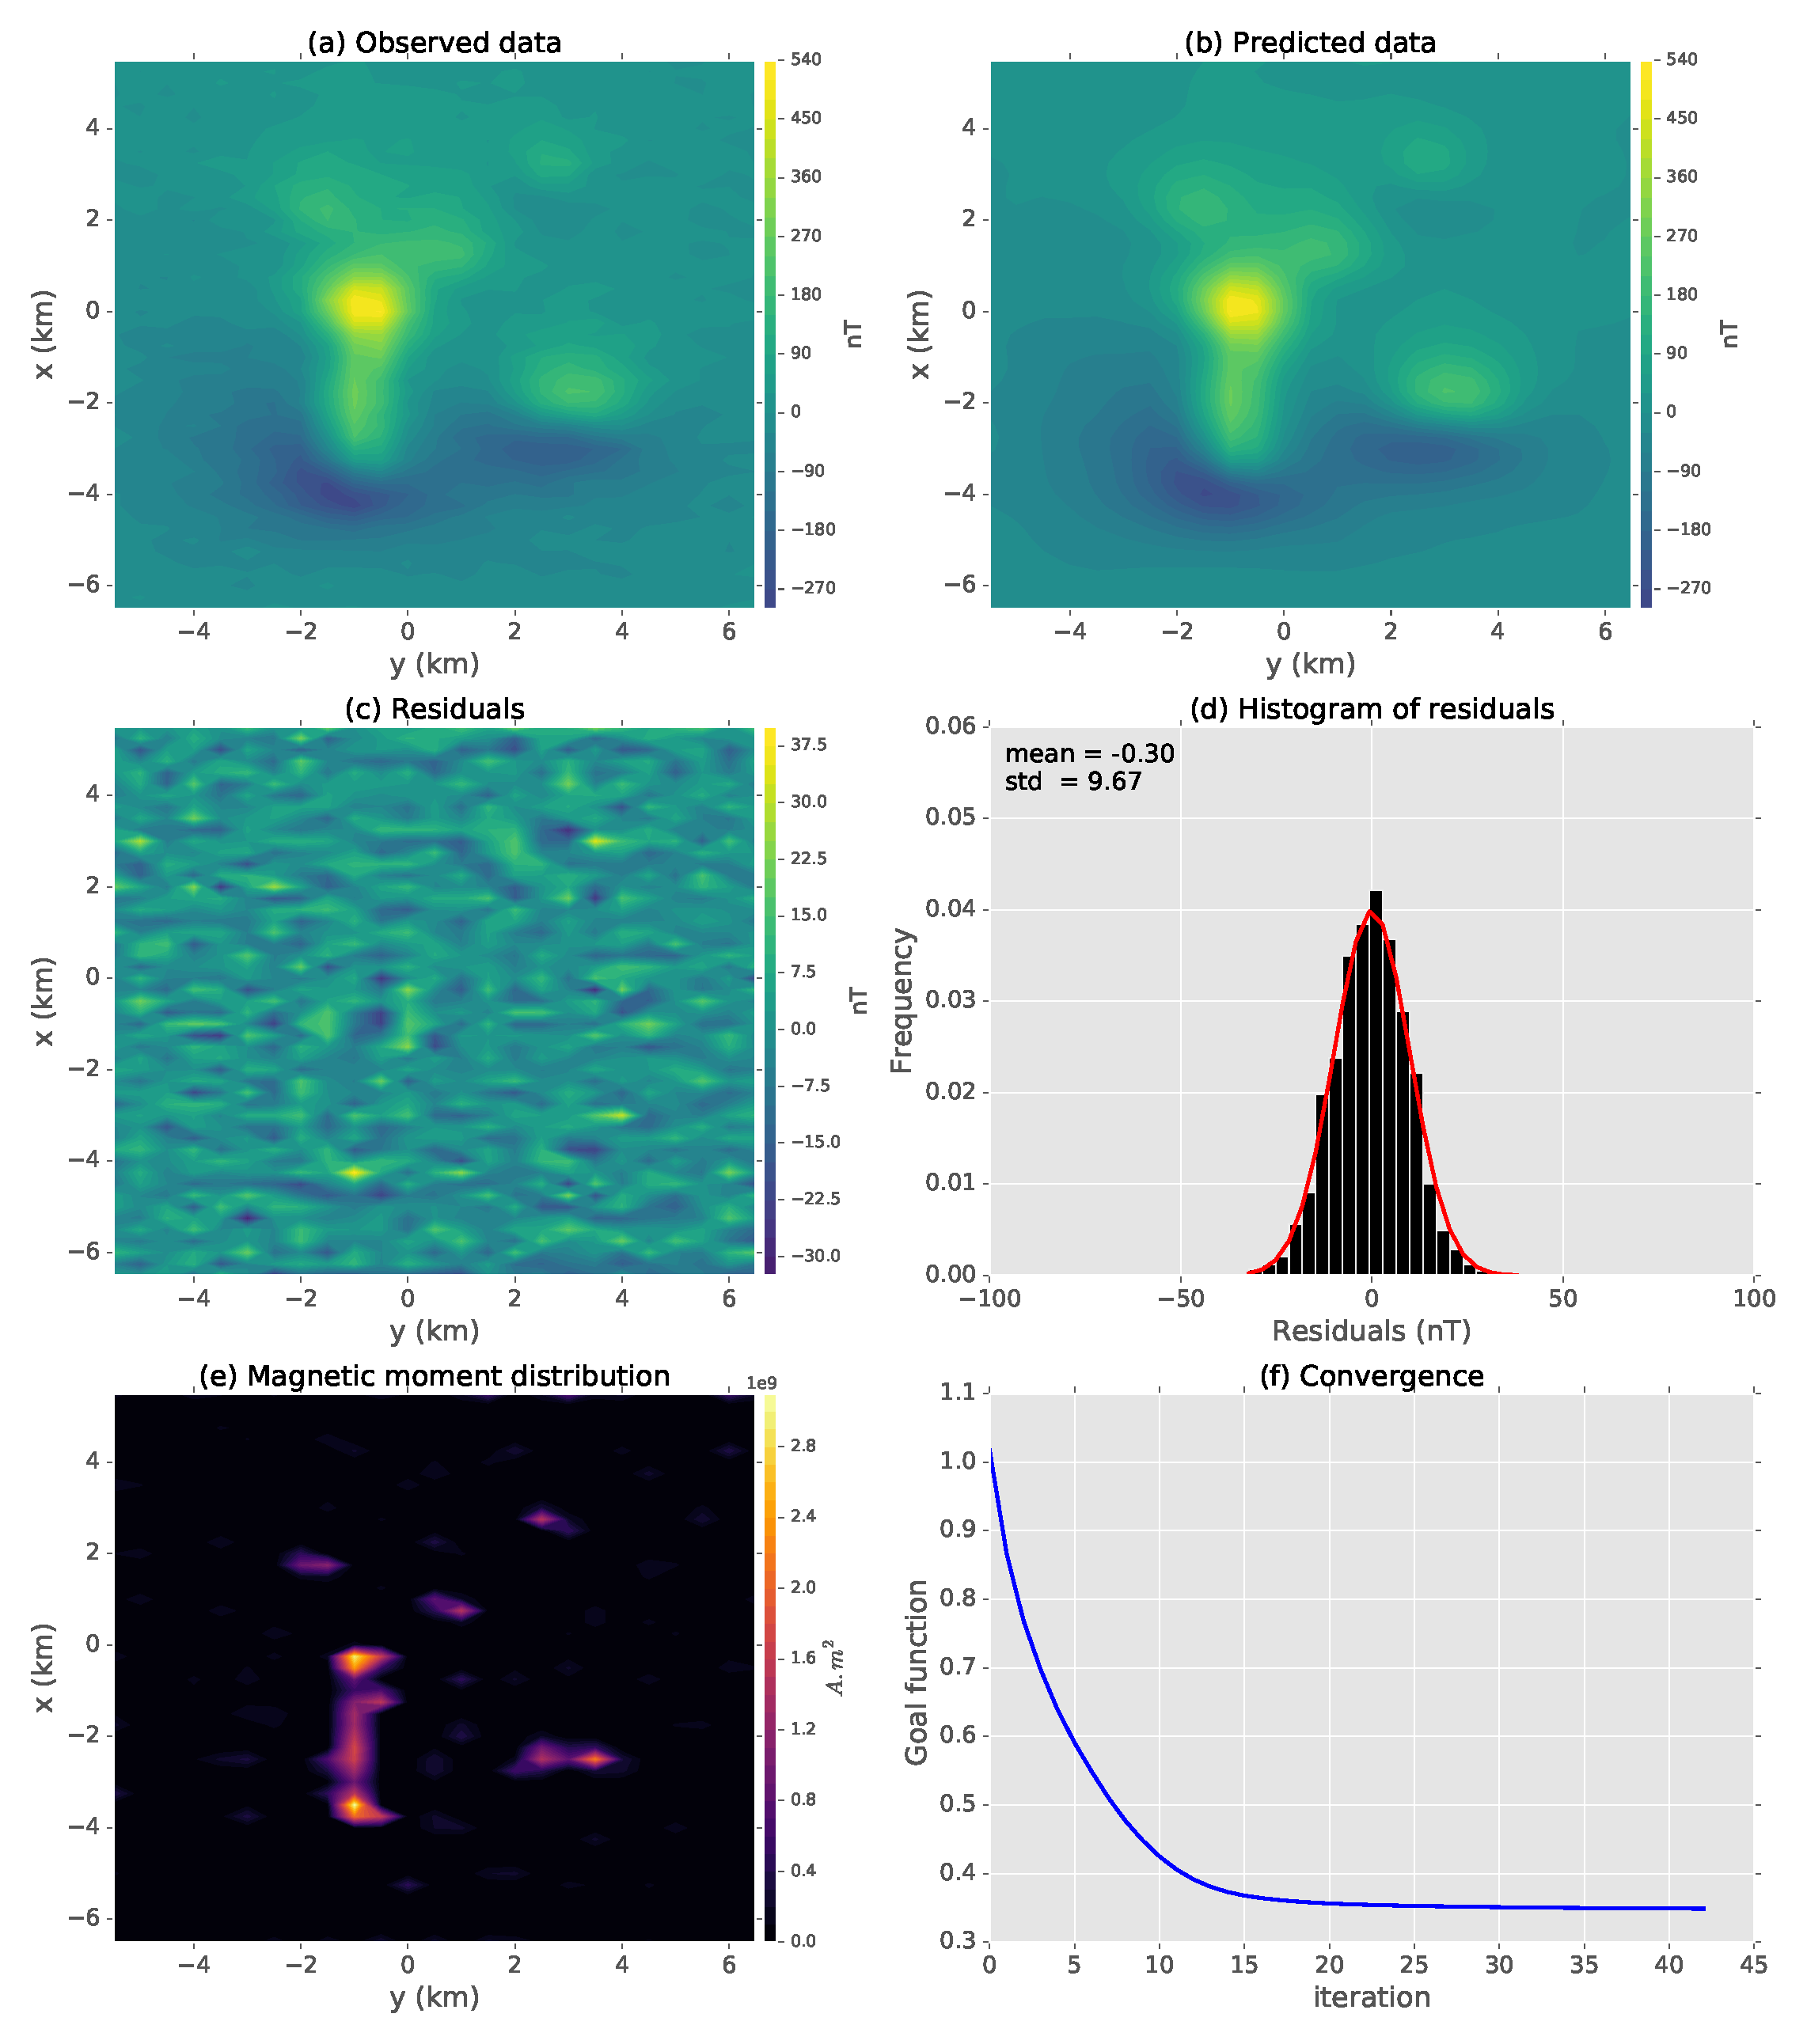
\includegraphics[width=0.85\textwidth]{Fig/unidir_test/results_compiled_LM_NNLS_magRM.eps}
	\caption{}
	\label{fig:unidir_test}
\end{figure}